\chapter{Odpowiedź skokowa}
Odpowiedź skokowa to odpowiedź układu na wymuszenie w postaci skoku jednostkowego w chwili $k=0$. Z powodu ograniczeń sterowania obiektu, skok jednostkowy jest niemożliwy, dlatego należy przeskalować odpowiedź skokową w następujący sposób:
\begin{equation}
\triangle{S_i} = \frac{S_i^0-Y_{pp}}{\triangle{U}}\textrm{, dla } i=1,\ldots,N
\end{equation}
gdzie $N$ to wybrana długość odpowiedzi skokowej.
\begin{figure}[tb]
\centering
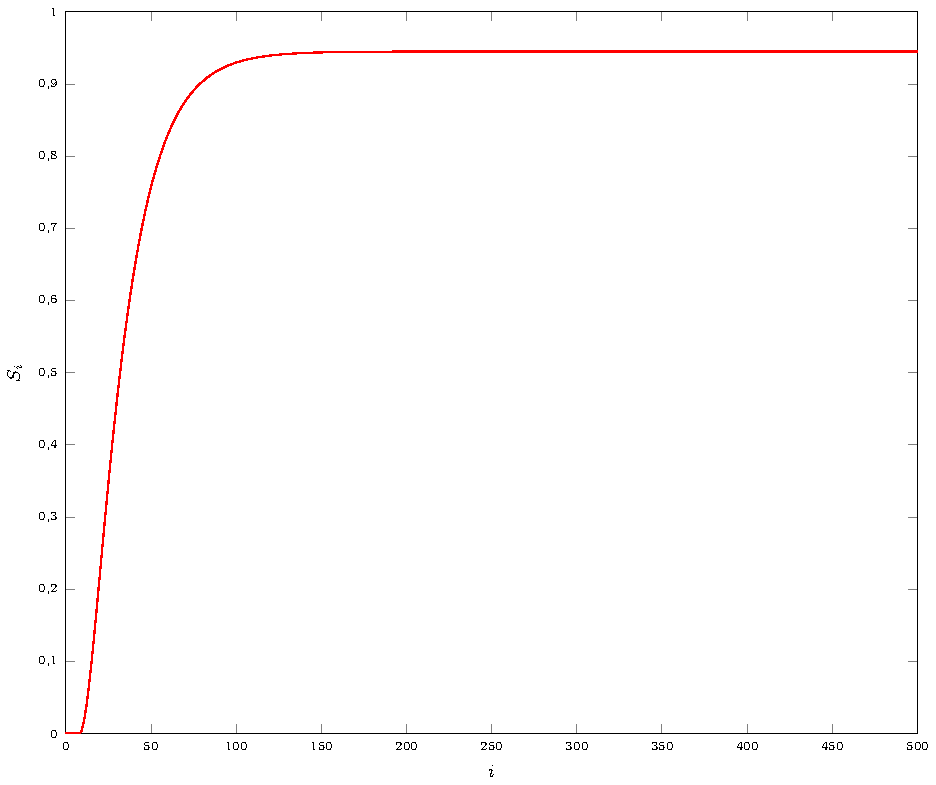
\includegraphics[scale=1]{wykresy/odp_skok}
\caption{Odpowiedź skokowa}
\label{odp_skok}
\end{figure}
Odpowiedź skokowa prezentowana na wykresie \ref{odp_skok} została otrzymana z przesklowania odpowiedzi obiektu po skoku z $u_{pp}=\num{1.1}$ do $u=\num{1.4}$.